%%
%% This is file `mcmthesis-demo.tex',
%% generated with the docstrip utility.
%%
%% The original source files were:
%%
%% mcmthesis.dtx  (with options: `demo')
%% !Mode:: "TeX:UTF-8"
%% -----------------------------------
%%
%% This is a generated file.
%%
%% Copyright (C)
%%     2010 -- 2015 by latexstudio
%%     2014 -- 2016 by Liam Huang
%%
%% This work may be distributed and/or modified under the
%% conditions of the LaTeX Project Public License, either version 1.3
%% of this license or (at your option) any later version.
%% The latest version of this license is in
%%   http://www.latex-project.org/lppl.txt
%% and version 1.3 or later is part of all distributions of LaTeX
%% version 2005/12/01 or later.
%%
%% This work has the LPPL maintenance status `maintained'.
%%
%% The Current Maintainer of this work is Liam Huang.
%%
\documentclass{mcmthesis}
\mcmsetup{CTeX = true,   % 使用 CTeX 套装时,设置为 true
        tcn = 0000, problem = B,
        sheet = true, titleinsheet = true, keywordsinsheet = true,
        titlepage = true, abstract = true}
\usepackage{palatino}
\usepackage{lipsum}
\title{The \LaTeX{} Template for MCM Version \MCMversion}
\author{\small \href{http://www.latexstudio.net/}
  {
\includegraphics[width=7cm]{mcmthesis-logo}}}
\date{\today}
\begin{document}




\section{Model 1: Two-dimensional Cellular Automata Model}
\subsection{Introduction}
In order to discover the influence of size, shape and merging pattern, we
 propose a two-dimensional Cellular Automata (CA) model. Our model is based on
 the one-dimensional \emph{Nagel Schreckenberg} model, which was first presented in
 1992 and successfully demonstrated many features of the traffic flow.

 Compared with a one-dimensional CA model, a two-dimensional one is more complex
 but feasible enough to simulate the real traffic flow. Therefore, the results
 from a two dimensional CA model is relatively more accurate.  Basically,
 the CA model can be regarded as an effective method to simulate features of
 traffic jams by showing how interactions between nearby vehicles cause the
 deceleration.
\subsection{Assumptions}
%用项目列表
\begin{itemize}
\item We assume that all the drivers are selfish
and short-sighted. To be specific, drivers always
adopt measures to move to the Roads Leading to Exit
(RLE), wherever they are.
\item We assume that once a vehicle leaves the
exit of the toll plaza, it will accelerate, namely
no congestion outside the plaza.
\item We assume that both the choices
towards tollbooths and the coming time of
vehicles satisfies random distribution.
\end{itemize}
\subsection{Model Establishing}
 In our two-dimensional CA model, each cell is
 evenly distributed in the shape of square. So the
 toll plaza, or rather, the whole departure area
 consists of plenty of square cells.
An independent cell or an adjacent cell cluster
can denote both empty roads or vehicles according
to their corresponding sizes, such as length and width.
We can assign a certain speed to each cell-formed vehicle.
But each speed value must be an integer, ranging from 0
to an identified $v_{max}$.
In addition, time is also discretized. Each time step
is defined as the time that a car takes to travel past
the length of 10 cars at the speed of the restricted
value.During a step interval, vehicles are set to perform
the following actions sent by corresponding instructions
in order.
Another important rule is that vehicles always perform
their updated actions at the same time.

Several actions are further explained as follows:
\begin{itemize}
\item \textbf{Acceleration:}

It reflects a characteristic
that vehicles tends to travel as fast as possible. Here,
this action obeys a rule as:

if $v_t<v_{max}$, then $v \rightarrow min(v_{t+1},v_{max})$
\item \textbf{Deceleration:}

 This action guarantee no
collision with the vehicle ahead. It satisfies:
$$v_t \rightarrow min(v_t, dx)$$
\item \textbf{Random deceleration:}

It embodies behavioral discrepancy of drivers. The
introduction of random deceleration basically reflects
the overreaction in decelerative processes. In conclusion,
it is a key factor that causes congestion. Likewise,
it meets following principle:

If $v_t > 0$, then $v_t \rightarrow v_{t-1}$ with probability $p_v$
\item \textbf{Steering:}

 It describes the trends that divers are more willing to
 turn to the Roads Leading to Exit (RLE) if they are not
 on the RLE at this moment. The corresponding rule is:

If (y\textgreater $W_L$), then $v_y=1$ with probability $p_y$

\item \textbf{Lane changing:} When a vehicle gets stuck,
the driver is likely to convert his or her lane to a n
earby one (only the one closer to the RLE) if that lane
is empty. It is also set to satisty:

If $dy\textgreater1$ and $v=0$, then $vy=1$ with
probability $p_d$

\item \textbf{Horizontal velocity:}
$$v_x=\sqrt{v^2 - vy^2}$$

\item \textbf{Motion:}

 It indicates that the position of a vehicle is
 shifted by its speed $v_x$ and $v_y$, thus,
 $x\rightarrow x+dx, y \rightarrow y+dy$

\item \textbf{Incoming vehicles:}

 Each vehicle will travel from the start of a
 certain tollbooth with the probability of $p_{in}$.
 This probability can denote traffic density in some
 ways.

 Where,

 % Table generated by Excel2LaTeX from sheet 'Sheet1'
 \begin{table}[htbp]
   \centering
   \caption{Add caption}
     \begin{tabular}{ll}
     \toprule
     $v_t$  & The speed of current moment \\
     $v_{max}$ & The maximum speed allowed \\
     $v_{t+1}$ & The speed of next moment \\
     $dx$    & The nearest distance between two nearby vehicles in their horizontal direction \\
     $dy$    & The nearest distance between two nearby vehicles in their vertical direction \\
     $p_v$  & The probability of randomlization \\
     $p_y$  & The probability of sheering \\
     $p_d$  & The probability of lane changing \\
     $p_{in}$ & The probability of incoming vehicles \\
     $v_x$  & The horizontal velocity \\
     $v_y$  & The vertical velocity \\
     $W_L$  & The exit width of the toll plaza  \\
     \bottomrule
     \end{tabular}%
   \label{tab:addlabel}%
 \end{table}%



\end{itemize}
\subsection{Simulation and discussion}
We convert our thoughts and design above into program instructions via Python,
and simulate a toll plaze with 8 tollbooths and 3 lanes of travel.

Common vehicles are usually $4-4.5m$ long and $1.65-1.85m$ wide,
so a vehicle will take up 2 cells.
According to the \emph{Green Book, 1994}, an appropriate design of
a toll plaze would be a trapezoid with a
168-meter-long recovery zone and a 612-meter-long departure zone.
The width of a tollbooth along with a toll island
is usually $5.5m$, while that of each lane is $3.5-4m$.
We set the length of each cell equal to $2m$: $l_{car}=4m$.
So the parameters are as follows:
\[
\begin{align*}
&{l}_{veh}=2m\\
&{W}_{veh}=1m\\
&W_{B}={W}_{b}B=3\times8=24m\\
&W_{L}={W}_{l}L=2\times3=6m\\
&{L}_{r}=84m\\
&{L}_{d}=306m
\end{align*}
\]



Figure~\ref{fig:q-p} shows the relationship between current throughput and
traffic flow density with different ${p}_{v}$.

%{翻译}当流量取得最大值q_max时对应的临界密度{d}_{c},zhegetu
%被临界midu划分为两部分,当流量小于临界密度dc时,车流为自由流.
%pv是随机减速概率,it varies between different drivers.figure shows that pv越小,对应的
%capacity 越大,dc也越大。在下面的章节里,我们主要采用了Pv=0.5来讨论,因为这时capacity约为700
%veh/h/lane,与实际情况个较为吻合

\begin{figure}[h]
\small
\centering
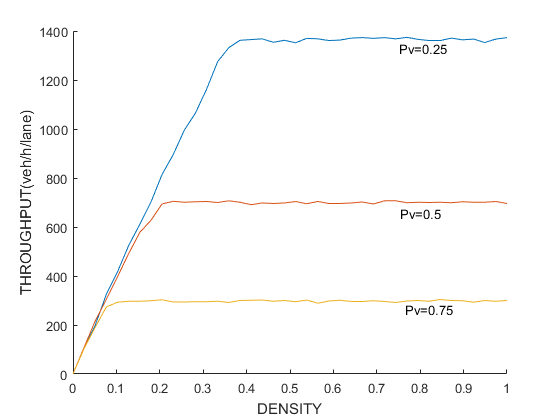
\includegraphics[width=12cm]{q-p-difPv.png}
\caption{The relationship between throughput and density with different ${p}_{v}$}
\label{fig:q-p}

\end{figure}

The density in the correspondence with the maximal throughput $q_{max}$ is
defined as critical density $d_{c}$. We can distinguish that the curves in
Figure~\ref{fig:q-p} are divided into two sections by that critical density.
If the flow density is lower than $d_{c}$, it will be a free flow (as Figure shows);%注意图片对应
 otherwise, a crowded flow (as Figure shows).%没写是图几
%插入两张图片free_flow&crowded_flow
We can conclude from the simulations above that the RLE are the most crowded
part once traffic density increases to cause congestion. In this case, drivers
always consider turning to the RLE as soon as possible, which causes unevenly
distribution of traffic density in the departure zone.


As mentioned above, ${p}_{v}$ is the probability of random deceleration.
It varies among different drivers. It is not difficult to conclude
that the smaller the value is, the larger $q_{max}$ is accessible. At the same
time, $d_{c}$ will increase correspondingly. In the following chapters, we
choose to adopt ${p}_{v}=0.5$ as our basis, because the $q_{max}$ at this time is
is consistent with the actual value, approximately 700 $veh/h/lane$. And more
detailed simulation results will also be displayed.





\end{document}

%%
%% This work consists of these files mcmthesis.dtx,
%%                                   figures/ and
%%                                   code/,
%% and the derived files             mcmthesis.cls,
%%                                   mcmthesis-demo.tex,
%%                                   README,
%%                                   LICENSE,
%%                                   mcmthesis.pdf and
%%                                   mcmthesis-demo.pdf.
%%
%% End of file `mcmthesis-demo.tex'.
